
%3/4 pages au moins en français (idem pour conclusion)
%\begin{itemize}
%\item fines échelles et leur rétroaction/structuration de circu générale
%\item choix région Gibraltar (Rencontre deux masses d'eaux, alimentation Méditerranée, outflow med)
%\item les fines échelles à Gibraltar (quels phénomènes (solitons, ressaut, etc))
%\item Outils de la thèse : num, obs (compagne,sat)
%\item état des lieux modélisation num fines échelles océaniques, problematique quantification mélange diapycnale
%\item plan
%\end{itemize}

Certains des éléments bibliographiques sont repris dans les introductions des différents chapitres, conçus comme des articles.

\section{Contexte}
\subsection{Dynamique océanique : vers les fines échelles}
(pose principes circu océanique, présente contexte des échelles généralement considérées en océanographie physique)

La circulation globale océanique, pilotée par les vents et le flux de flottabilité, s'organise en un ensemble de courants de grande échelles (gyre, AMOC,...) qui en parallèle et en interaction avec la dynamique de l'atmosphère, transporte la chaleur. \\
\color{red}
Margaux, voici une proposition de figure illustrative pour cette partie de ton introduction... Nous pouvons la modifier et l'adapter un peu ensemble mercredi matin si tu veux et je peux t'écrire un premier jet de présentation que tu ferras tien ensuite... Elle n'a pour le moment pas été publiée mis à part dans mes dossiers de "carrière" (trucs inutiles que personne ne lit). Aucun problème en ce qui me concerne pour que tu te l'appropries d'une façon ou d'une autre dans ton manuscrit si tu partages ce qu'il y a dessus bien sûr. L'idée est justement de présenter de façon très schématique les différentes "cascades" et en parallèle les différents modèles de turbulence (enfin ceux qui m'ont semblé les plus importants en tout cas) pour déboucher sur une définition des fines échelles justement. \\
Si cela te convient... Cela veut dire que je peux prendre le relais sur les parties 1.1.1 et 1.1.2 pour te faire une première proposition pendant que tu continues sur 1.1.3 et suivantes. Dis-moi ?\\
\begin{figure}[!h]
  \centering
  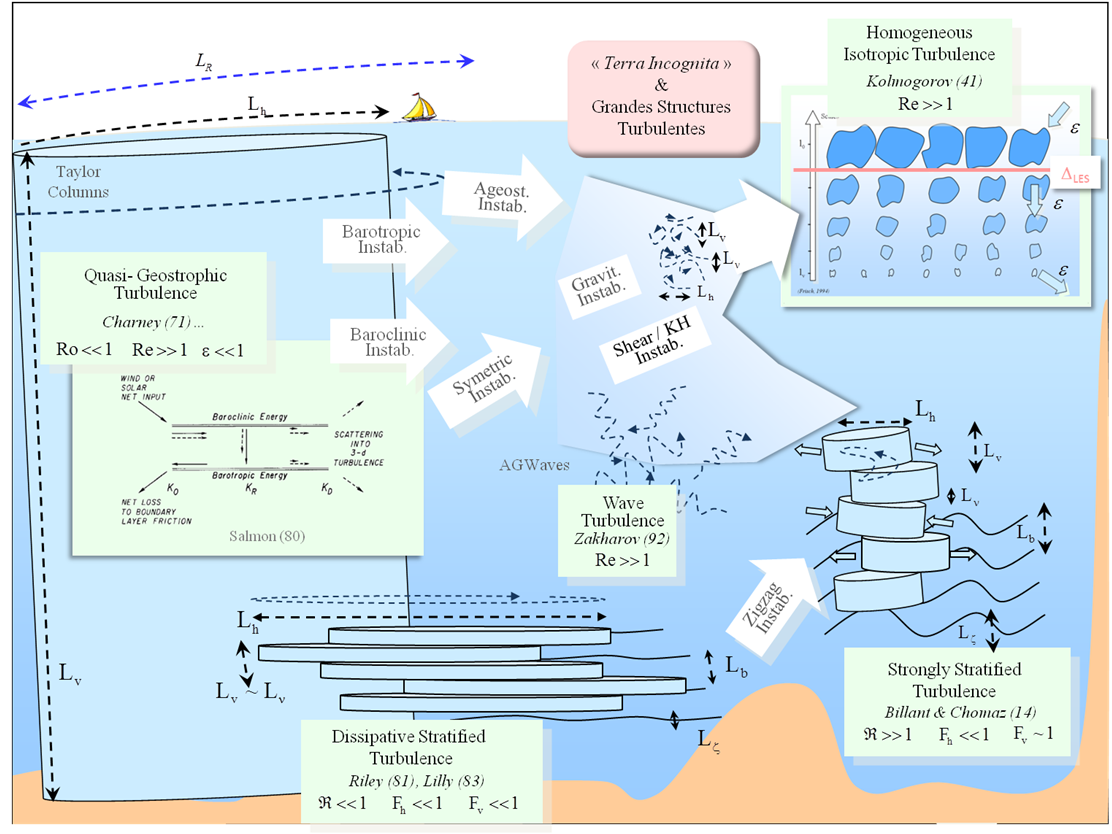
\includegraphics[width=0.8\textwidth]{./INTRO/Ocean_scales.png}
  \caption{\color{red}l'océan vu à travers ses cascades d'échelles, ses instabilités et ses principaux modèles de turbulence.\color{black}}
  \label{fig_ocean_scales}
\end{figure}
\color{blue}
L'océan est soumis à de nombreux forçages, en particulier à travers sa surface libre mais pas seulement: forçages "mécaniques" par la pression atmosphérique, les marées astronomiques ou les flux de quantité de mouvement induits par le frottement du vent, forçages "thermodynamiques" par les flux de chaleur radiatifs ou par les flux de chaleur latente, forçages par les précipitations, les fleuves ou encore par évaporation... Ainsi présenté, l'océan est donc un \textit{système dynamiquement ouvert}, l'ensemble des forçages auxquels il est soumis induisant un large spectre de processus dynamiques: houle, courants d'Ekman, upwelling ou downwelling, ondes de marée, marées internes, convection profonde, courants de gravité, panaches fluviaux... \\
L'océan ne résume toutefois pas non plus à une somme de processus dont la combinaison linéaire suffirait à expliquer sa dynamique propre. Ces processus interagissent entre eux induisant d'importants \textit {mécanismes de transferts} entre les différentes gammes d'échelles spatiales et temporelles composant cette dynamique. Lorsque ces transferts prennent une forme cohérente dans des régions spécifiques du spectre, on parle de \textit{cascades d'échelles}. Les mécanismes débouchant sur ces transferts sont quant-à eux généralement associés à des \textit{instabilités dynamiques}.\\
Les cascades d'échelles ne débouchent pas nécessairement sur des structures dynamiques d'échelle réduite. Pour des échelles spatiales plus grandes que le premier rayon de Rossby, \cite{salmon_baroclinic_1980} (figure \noparref{fig_ocean_scales}) schématise les interactions sous la forme d'une \textit{cascade inverse} associée à des transferts énergétiques dirigés en moyenne sur la verticale majoritairement vers les plus grandes échelles alors que les transferts d'enstrophie sont quant à eux majoritairement dirigés vers les plus fines échelles. Les vents et les flux de chaleur induiraient ainsi des structures dynamiques de plus grande échelle qui par \textit{instabilité barocline} seraient brisées avant d'être transférées vers les plus grandes échelles "barotropes" et d'être dissipées par frottement dans les couches limites...

\color{black}

Cependant, l'océan (tout comme l'atmosphère) a un écoulement turbulent, c'est-à-dire chaotique et non-linéaire/ constitué d'une intéraction d'échelle.

...

Cette turbulence se manifeste en la décomposition des structures de grande échelles/synoptiques en des champs de plus petite structures/structures de plus en plus petites (transiant?) en intéractions les unes avec les autres (tourbillons, etc). Ainsi l'étude de l'océan peut se faire à bien des échelles spatiales et temporelles

Ce manuscrit de thèse porte sur l'étude d'une dynamique dite de 'fine échelle', sur les processus / phénomènes océaniques . Il s'agira 

\subsection{Turbulence et rétroactions}
(Revient plus en détail sur la turbulence, cas où mot est utilisé (turbulence géostrophique? vs cascade turbulente))

Turbulence de mésoéchelle (instabilité barocline), ici on s'intéresse au début de la cascade turbulente directe définie par Kolmogorov. Les 2 sont similaires en ce qu'elles concernent le transfert d'énergie vers de plus fines échelles. Pour le cas de la turbulence de fine échelle, // mais va aussi aboutir à structuration de l'écoulement en lui-même. (La conservation de la vorticité potentielle (PV) peut agir comme un effet structurant de jet/courants...//méandres d'un jet / courant structurés par la conservation de la vorticité potentielle... PV générée par diabatic processes (in boundary layers?)...

...

Les grandes structures turbulentes marquent l'entrée de la cascade directe menant à la dissipation moléculaire. Elles sont ainsi à l'origine d'une réorganisation irréversible, diabatique de la colonne d'eau et les "traceurs" passifs ou actifs sont redistribués dans l'océan. Parmi ces "traceurs", la masse volumique1 joue un rôle particulier dans la dynamique océanique: les masses d'eau sont par exemple "transportées" le long des surfaces isopycnales et le contenu en vorticité potentielle entre deux de ces surfaces isopycnales se conserve au cours du temps2.

...

Les talus continentaux, dorsales océaniques, monts sous-marins isolés, détroits... sont autant d'accidents bathymétriques qui canalisent, perturbent, modifient la circulation et plus généralement la dynamique océanique. Les accidents bathymétriques sont localement le siège de régimes de couches limites particuliers entraînant quasi-systématiquement l'apparition de structures turbulentes et ouvrant ainsi les portes de la... "terra incognita".

...

Les ondes internes de gravité ont, jusqu'à ce jour, occupé une place à part dans mes travaux de recherche. Sous la forme de rayons se propageant et se réfléchissant sur le fond, la surface libre ou la pycnocline, sous la forme d'ondes solitaires de grande amplitude se propageant le long de la pycnocline océanique ou encore sous la forme de modes 1, 2 ou 3 sur les plateaux océaniques... ces processus jouent un rôle particulier dans l'océan et plus spécifiquement dans la redistribution de l'énergie. Leur déferlement, leur instabilité donnent généralement naissance à des "patchs turbulents" annoncés par l'apparition de grandes structures turbulentes.

Cascade inverse???

\subsection{Le Détroit de Gibraltar}
(intérêt de la zone en vu du blabla précédent)



\section{L'étude des fines échelles/connaître/etc...}
(verrous puis objectif)
\subsection{Une dynamique difficile à appréhender, à quantifier}
Ici parle BPE

\subsection{La simulation numérique}
En simulation... physique couplé numérique

...

Le démonstrateur Gibraltar ouvre en quelques sortes la boîte de pandore alors que nous sommes sur le point de franchir une étape clé pour la simulation de la dynamique océanique. CROCO permet en effet de basculer dans cette partie du spectre océanique complexe et mal connue (car difficile à observer) qu'est la "terra incognita". Les grandes structures turbulentes dont il est en particulier question ici sont le résultat de diverses instabilités "primaires" peuplant la méso et la sous-méso-échelle océaniques (Fig. 1): instabilités barotrope, barocline, symétrique, zig-zag, agéostrophique, paramétrique des ondes internes, etc... Ces mécanismes de déstabilisation peuvent être vus comme brisant des structures, des processus, des équilibres subtils régissant localement et de façon éphémère la dynamique de l'océan. Ils sont généralement (mais pas exclusivement) la première étape d'une déstabilisation en cascade basée sur des instabilités de cisaillement et des instabilités convectives. Ces mécanismes souvent non-linéaires et complexes étaient jusqu'à peu l'apanage des modèles "sous-maille". N'étant par conséquent pas universels, ces derniers rendent la simulation très dépendante du lieu et de la période étudiés: les "modèles de fermeture" doivent en effet être ajustés et confrontés à la réalité avec comme principal enjeu le choix du modèle et la détermination des paramètres physiques ou numériques qu’il inclut nécessairement. Si ces grandes structures turbulentes sont à portée de modèles comme CROCO dans l’océan intérieur, elles demeurent par contre hors d’atteinte dans les couches limites de surface et fond, régions dans lesquelles leurs échelles spatiales caractéristiques peuvent considérablement décroître.

...

Terra Incognite : A. Scotti (Scotti, 2010), dans une revue sur la modélisation de l'océan, reprend la conclusion de J.C. Wyngaard (Wyngaard, 2004) rédigée quelques années auparavant pour l'atmosphère et explique qu’avec la représentation explicite des grandes structures turbulentes, la simulation numérique entre en "terra incognita". La "terra incognita", souvent aussi qualifiée de "zone grise" ou « fines échelles océaniques », est plus largement considérée ici comme cette région particulièrement mal connue du spectre océanique où la dynamique peut localement et temporairement basculer d'un équilibre simple entre un nombre limité de processus vers une dynamique non-linéaire complexe induisant une cascade d'instabilités dynamiques. Cette cascade d’énergie (directe) aboutit à la dissipation moléculaire.

...

Ces grandes structures turbulentes se développent de façon hétérogène à petite échelle (à priori quelques dizaines de mètres au maximum) et demandent donc un nouvel effort de réduction du coût de calcul. CROCO est en effet conçu et développé pour être un code efficace mais ce qu'il est aujourd'hui possible de simuler explicitement dans un détroit d'extension réduite doit être généralisé à des sous-bassins et à des plateaux continentaux de plus grande extension avec, très vraisemblablement, une résolution raffinée. Nous avons mené à bien une première étude de faisabilité au sein de notre petit groupe CROCO / LA débouchant sur le portage du code sur GPU sur des machines hétérogènes CPU / GPU. Le nécessaire travail d’optimisation des performances est désormais en conduit en très étroite collaboration avec les équipes INRIA1. Le surcoût de calcul associé à la compressibilité et à la remise en cause de l'hypothèse hydrostatique a par exemple dors et déjà pu être effacé en déportant sur GPU l'intégration du mode rapide compressible.

...

La promesse d’une puissance de calcul pétaflopique puis exaflopique a, en théorie au poins, ouvert les portes de la simulation des grandes structures turbulentes (LES) pour l’océan et l’atmosphère. Les météorologues ont par exemple rapidement su tirer parti des moyens de calcul disponibles : des algorithmes dédiés ont vu le jour dès le début des années 2000 débouchant sur des codes numériques tels que WRF en version compressible ou Méso-NH en version anélastique. Ces deux types de codes permettent, chacun avec leurs spécificités, d’aborder la simulation de la cascade turbulente directe en représentant explicitement les plus grandes structures turbulentes dans l’atmosphère.

Les modèles océaniques n’ont pas été immédiatement en mesure de passer ce cap de la LES en grande partie à cause de la présence d’une surface libre aux conséquences dynamiques multiples. Cette surface libre rend en particulier plus complexe la relaxation de l’hypothèse hydrostatique. Dans la foulée de l’ANR COMMODO rassemblant au milieu des années 2010 l’ensemble des équipes françaises travaillant sur la modélisation de l’océan, nous avons décidé de faire rapidement évoluer nos codes numériques vers une nouvelle génération de codes capables d'explorer cette "Terra Incognita"1 (Fig. 1) que constitue la "zone grise" associée aux grandes structures turbulentes (Scotti,2010; Wyngaard, 2004). Nous nous sommes pour cela associés pour développer le code CROCO au sein d’une véritable « équipe de recherche » rassemblant chercheurs en océanographie et en mathématique (analyse numérique). Un Groupement de Recherche éponyme est né associant l’université de Toulouse et les principaux organismes de recherche en informatique et en océanographie français: l’IRD, INRIA, le CNRS-INSU, l’IFREMER et le SHOM. En 2021, l’IRD a entériné la constitution d’un GdRi1 CROCO tourné vers nos partenaires au Sud. Une première étape était ainsi franchie confirmant les fructueuses collaborations déjà bien en place.

Cette réflexion de fond et les développements sur lesquels elle a débouché nous placent quelques années plus tard dans une position de pionniers au niveau international. Notre outil de modélisation d’océan CROCO et sa communauté de physiciens et de numériciens est actuellement unique aux échelles régionales, côtières. Même si le code CROCO n’a pas encore atteint le degré de maturité du code national NEMO, les communautés CROCO et NEMO ont en outre commencé à bâtir sur leur forte complémentarité en termes d’échelles spatio-temporelles simulées. L’ANR COMODO avait ouvert la voie à la mise en commun de savoir-faire débouchant sur des projets communs : études amonts de la DGA, développements méthodologiques autour de l’équipe AIRSEA d’INRIA ou encore mise en commun d’outils de modélisation: XIOS, NEMOVAR...

\subsection{Démarche de la thèse}
Les années de thèse ont eu pour objectif de mettre en place outil sur une région particulièrement/// Simuler explicitement, observer, quantifier, pour explorer intéraction d'echelles sur spectre élargi


\section{Plan du manuscrit}




%Morceaux de intro GBR3D : 
%The amplitude of the exchange varies over timescales larger than the semi-diurnal tide. The lower frequencies (whether seasonal or inter-annual) are usually linked to atmospheric forcing over the Mediterranean \citep{sanchez-roman_2012}. The tidal eddy-fluxes have their own variability associated to the spring-tide cycle and to the monthly tides, with for example a greater depth and stronger shear during neap tides, but more intense mixing during spring tide \citep{naranjo_2014,vargas_2006}.\color{red}(enlever? sert à rien? que dans intro plus générale???)\color{black}


%Numerical models are discretized and have a treshold resolution under which phyisical pehomenons cannot be represented explicitely. Particularly, diffusion and ... processes,  among other parametrisations of processes like surface exchanges, radiation that occur at molecular or submolecular scales. Diffusion and dissipation are molecular in nature as a , energy flux, but more broadly speaking, dissipation is the transfer of energy from great scales to small scales. In a stratified fluid, this dissipation is accompagnied by mixing , ie a lewoering of potential energy, or more accurately and explained i paragraph ..., of the background potential energy.
%Broadly for oceanic (or more generally geophyisic?) models classification on DNS, LES, and RANS. DNS has molecular dissipation
%For the discussions simply coining as LES is not sufficient but need to precise LES in regard to which phenomenon. For exemplein chapoter ... of this manuscript, coined LES because primary instabilities of the flow. However, the primary instabilities that are known to exist at upper and lower boundaries of teh water column are not represented and are parametrized, so in regard to the dissipation those process not LES. 
%To this considerations, one must also not forget that the discretisation itself introduces numerical dissipation unless using centered schemes (computationnally impossible).



%\subparagraph{Conclusion générale/dans le manuscrit}
%Les simulations ... sont première LES maisblablablablabla (trad ce que avait dit...). Besoin outil diagnostique du mélange, chapitre prochain...



